\chapter*{Complexity: An Existential Threat to Effectiveness}
\addcontentsline{toc}{chapter}{complexity} 
%\openepigraph{%
%Any fool can know.\\ The point is to understand.
%}{Albert Einstein}

\openepigraph{I must not fear. Fear is the mind-killer. Fear is the little-death that brings total obliteration. I will face my fear. I will permit it to pass over me and through me. And when it has gone past I will turn the inner eye to see its path. Where the fear has gone there will be nothing. Only I will remain.}{Frank Herbert, Dune}

\marginnote{
	\newthought{Key Takeaway:} Complexity is making public health less effective than it might once have been and it is seen to be less effective. Our inability to step outside our analysis paradigm is, I believe largely responsible for the situation. It has become so ingrained it is 'thinking', and we compound the ways-of-working that make it ever more difficult to escape. 
}

\newthought{Complexity}: Whenever I talk or present on the subject of complexity, I am reminded of Dune, a Frank Herbert created universe in which its Bene Gesserit repeat the above as a litany against fear. Subconsciously, I insert 'complexity' after 'fear'. I can hear an inner voice saying it... There is no other public health topic that provokes such strong aversion. It really is a mind-killer! The public, colleagues, politicians -- almost everyone will walk a long road to avoid having to deal with it.

It would be hard to argue that our world isn't complex; and, I have yet to ever hear a colleague state that they would like their organisation to be less effective. These are modern day 'motherhood statements'. Almost everyone would agree, and almost no one seems to be doing anything about it. It is easier to agree with this statement than it is to understand the implications. Maybe the key sticking point is the word 'requires'.

Complexity 'requires' more effective practice. Does it? Why? What is wrong with the current practice of public health? Well there are a couple things wrong. First, our practice is 'reactive' -- we see events (deaths and illness) and then we react to their occurrence. Secondly, we focus on the event itself and we rarely explore why the event occurred beyond the most proximal causes. Thirdly, and most bizarrely, we treat almost every illness as if it was a 'stand alone' problem, not at all related to any other form of ill health. In fact, we've organised not only public health practice around this idea, but our health systems and even the study of medicine are organised into disease specific silos. 

If effectiveness is the degree to which your organisation achieves its desired outcomes or results, who wouldn't want their organisation to deliver more effective public health? I've never worked in a public health organisation that couldn't have achieved more than it was actually delivering. If '0' represents achieving nothing (zero effectiveness) and '100' achieving everything (perfect effectiveness) -- how do you rate your organisation?  

Typically, a public health organisation's approach to being more effective is to attempt new types of intervention, or if it all seems to be getting a bit desperate we'll restructure our organisation or even our health system! So we already expend a lot of resource on trying to be more effective. How's that working out for your organisation? It seems a bit hit and miss, doesn't it? Moreover, this doesn't address the key limitations of current practice: reactiveness, proximal focus and silo view of the world.

If you are a colleague interested in public health outcomes, this book will help you understand how to identify effectiveness gains and build them into the fabric of your organisation. This is nothing less than transforming the way organisations think, do and learn. I hasten to add that I'm not advocating burning-the-house-down and rebuilding, but rather about modernising the old property by putting in a new windows so that we can see more of the outside and let more light in.

\section{A journey into health systems complexity}

In the mid-1980s, years before I knowingly found my 'public health' career path, I landed an incredible summer government internship monitoring agricultural pesticides in the ground water of Southern Ontario, Canada. It was incredible, because it had everything: It used almost everything I was learning in my Geography undergraduate programme and it provided a real world application of all this learning. I thought that was pretty cool, and I knew I was very lucky. After many years of hospitality jobs, I was doing something that I felt for the first time could be the start of a career path! Not only that, they gave me a car, there was an expense account for lunches, and all I had to do was drive around in the sun with the windows down, the radio turned up and visit my list of farms each week over the summer and take a sample of water from an outside tap.

This 'first real' job, as I felt back then, has long dropped off my CV. I would only remember the fun I had these many years later, were it not for the fact that my boss at this government agency encouraged me to do the research year of my honours degree on the programme I was working for, so my very first real job is documented by my 79 page, leather bound 'undergraduate dissertation'. No one has ever cited this research to my knowledge, so let me be the first\cite{Skelly1988}.

The monitoring programme ended up running for three or four years, but  because of the concerns it began to generate. The first summer, and the one I based my undergraduate thesis on, had not identified the target pesticide, Alachlor nor its metabolites, and we only had a few regularly positive wells for the most widely used pesticide Atrazine and it's metabolites. Consequently I went with the flow and took a slightly wider focus for my academic research: 

 very few wells that we monitored showed any contamination, but many more wells were found to be contaminated during the second summer. By the third summer most wells were contaminated. 

We were sampling drinking water wells on farms and, as you can imagine, this was a 'problematic situation' to put it mildly. These wells were largely defined as being shallow and in unconsolidated sand and gravel aquifers. Exactly the type of wells that you would expect to see pesticide contamination in if the pesticides were getting into the soils and down into the groundwater. 

However, what you really need to know was that this didn't seem to be related to the introduction of new pesticides or any change of practice on farms relating to how pesticides were sprayed, when they were sprayed or how the soils were fertilised or ploughed. The crop cover was largely static. Nor did it seem that changes in rainfall could explain the changes. Blame complexity.

In fact, when we started seeing more wells contaminated in the second summer, it was well understood what was happening. The problem happened before the groundwater sampling for pesticides even began.

\section*{The great health thought leaders and their challenges}

%\section{Structured for a simpler time - how public health practice needs to change}
\subsection{A simpler time}
The start of modern public health practice is often pegged to the work of John Snow during the cholera outbreaks of 1840s London, about 180 years ago. For the next 100 or so years, the focus of public health was on infectious disease.

The John Snow story reminds us of the importance and effectiveness of the 'hygiene revolution' delivered by sanitation engineering. Separating drinking water from waste water in urban environments, and then eventually cleaning both has had a dramatic impact on population health.

Prior to 1960, we could probably say that public health practice had three foci:
\begin{enumerate}
	\item Sanitation \& Hygiene: Drinking water, waste water, hand washing
	\item Vaccination: Smallpox, anthrax, rabies, typhoid fever, cholera, tuberculosis, polio
	\item Control of communicable disease: isolation, quarantine, vermin and disease vector control
\end{enumerate}

We tackled problems as they came. With this limited array of tools, public health practice delivered unambiguous results. 

\subsection{An epidemiological transition}
\newthought{epidemiological transitions} are crucial concepts and the last one especially so because it marks the point at which we lost almost all of our effective tools -- they were useless against the rising tide of chronic disease. Sometime after the Second World War, maybe the 1960s, and it seemed that we had almost conquered infectious disease, public health turned its attention to chronic diseases (often termed 'non-communicable' diseases).

The emphasis went from doing, from engineering, from physical interventions as the way to deliver results -- to the processing and sharing of information and knowledge. The 'new' enemies are cancers, cardiovascular diseases including stroke and diabetes, chronic respiratory diseases, dementia, mental ill health, musculoskeletal disorders, immune system dysfunction, substance abuse, and many others, which are all influenced by the
\begin{itemize}
	\item Environment: air, water and noise pollution, weather and climate, nature and biodiversity, food system
	\item Conditions of living: local economy, economic resources, meaningful employment, housing availability, security and quality, public safety and crime, education and opportunity for development
	\item Lifestyle \& behaviours: social networks, family, substance abuse, exercise, stress, diet, sleep
\end{itemize}

I have been pondering three fairly fundamental questions of the 'practice of public health' that I'd like the reader to consider. How do we:
\begin{enumerate}
	\item Build a more effective systems-based \emph{Public Health} practice?
	\item Enable new ways of working that lead to more effective practice?
	\item Reimagine our system of learning beyond individual continuing professional development?
\end{enumerate}



\newthought{Most recent edits stop here}



Public health intelligence has two fundamental challenges: (1) Identifying the right questions, often generated elsewhere in the organisation and (2) answering these questions. We've not made significant advances on these two challenges over the 25 years or so that I've been involved in public health intelligence. The reason, in words attributed to Albert Einstein, is that

\begin{quote}
	\centering 
	\emph{We cannot solve our problems}\\ 
	\emph{with the same level of thinking that created it.}
\end{quote}

We have only one intelligence process that is widely used and that is 'analysis'. All modern evidence-based health and care systems are designed, run and supported using this fundamental process. If we are going to have any chance of tackling our two key intelligence challenges, we need to rethink our approach to problem solving.


\subsection{Rethinking Our Approach}

I believe that a mature intelligence function, in any type of organisation, should support critical problem-solving wherever that happens within an organisation or even across health and care systems. Intelligence processes need more depth; they need to be able to directly address the our key challenges. I propose the use of three interdependent problem-solving approaches be adopted by the organisational intelligence function (Table~\ref{tab:response}).

\begin{table}[h]
	\begin{center}
		\footnotesize%
		\begin{tabular}{p{1.75cm} p{2.75cm} p{4.75cm}}
			\toprule
			Intelligence processes & Problem-solving approaches & Principal output \& outcome for each problem-solving approach \\
			\midrule
			Analysis    & Analytical Thinking & Provide operational information\\
			& & Improved Knowledge \\
			Synthesis & Systems Thinking & Identify and frame critical problems \\
			& & Shared-understanding of why problems are occurring now \\
			& Futures Thinking & Compare multiple strategic directions \\
			& & Shared-understanding of routes to the most desired future states \\
			\bottomrule
		\end{tabular}
	\end{center}
	\caption{A layered approach to problem-solving in public health intelligence would include Synthesis, which provides two additional approaches.}
	\label{tab:response}
\end{table}

Public health intelligence might be unique practice within our health system for having no academic home, no single discipline. The fact that public health analysts are drawn from many disciplines is a strength when building teams, because intelligence groups are in general less vulnerable to disciplinary blind spots, which is why I think that intelligence functions should be about more than data, information and knowledge. Any small group with a plurality of perspectives should be thought of as organisational problem-solving facilitators. More on that later, but intelligence functions are a natural home for organisational process of synthesis (Figure~\ref{fig:apptosensemaking}).

\begin{figure}
	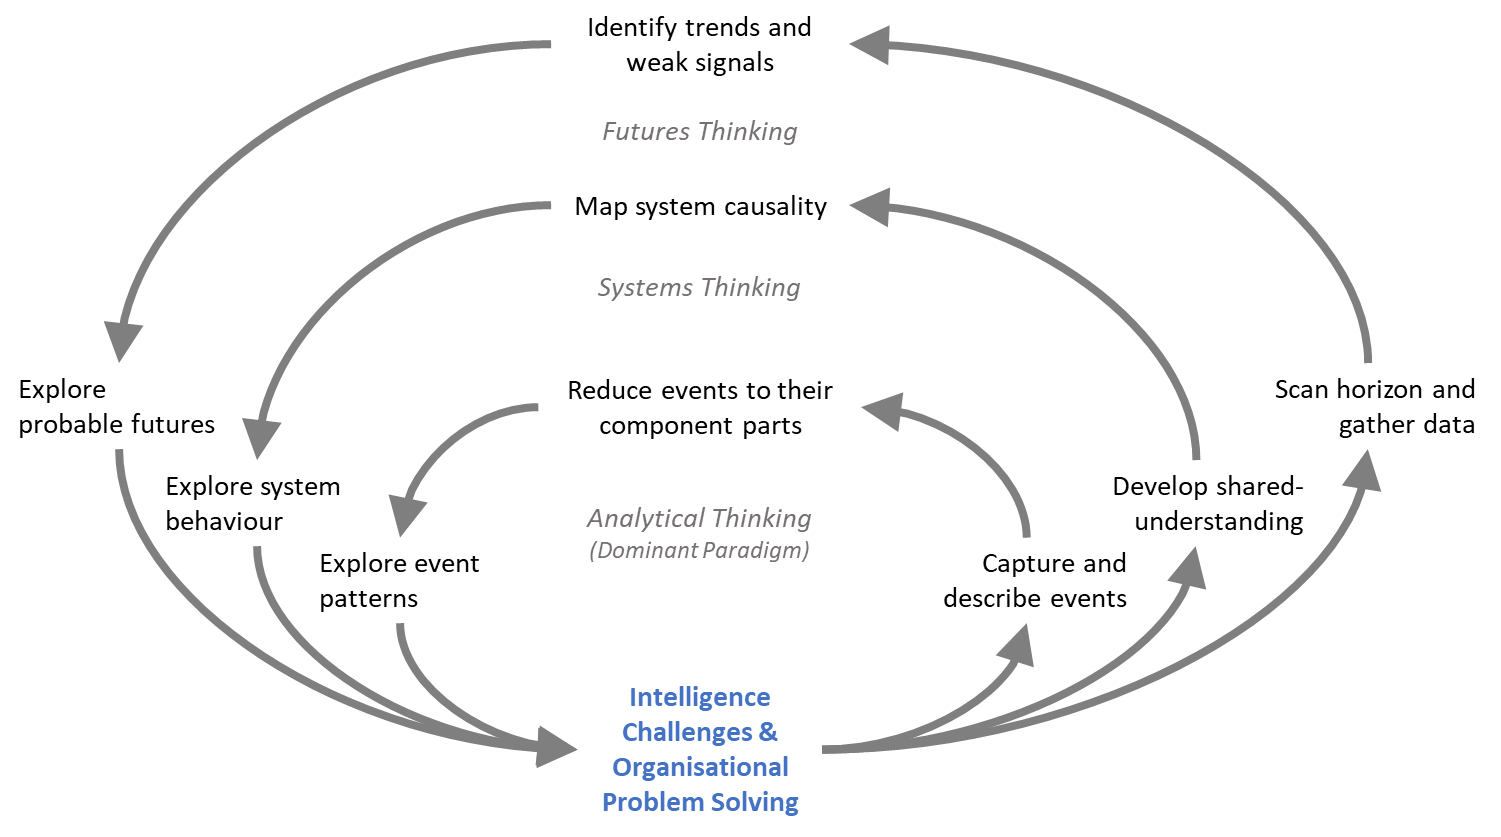
\includegraphics{./figures/approaches.png}
	\caption[Systems and Futures Thinking][6pt]{Systems and Futures Thinking, missing from all but the most mature intelligence programmes, effectively deepen the problem-solving capability of an organisation, by directly addressing the two key intelligence challenges. }
	\label{fig:apptosensemaking}
\end{figure}

My theory-of-change for the intelligence function itself suggests that if we transition our problem-solving from a single approach to three interdependent approaches we will ultimately increase the effectiveness of any public health organisation or health and care system of which we are a part (Figure~\ref{fig:toc}). While this premise is straight-forward, the purpose and implementation of these additional capabilities is a longer journey that I hope many of my colleagues will be keen to explore with me.

\begin{figure*}[h]
	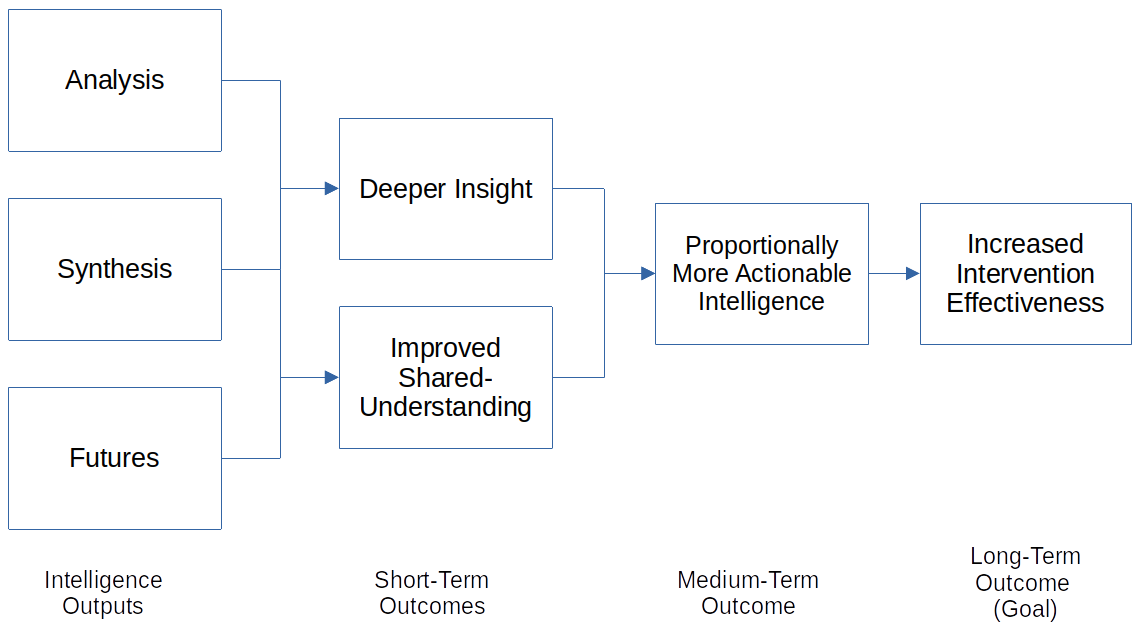
\includegraphics[width=\linewidth]{./figures/toc.png}%
	\caption{The premise underlying this book is encapsulated in this very simple theory-of-change. This same premise should underlie every mature intelligence process.}%
	\label{fig:toc}%
\end{figure*}


\section*{A public health intelligence perspective on the need for change}
I am a scientist by training and a public health intelligence 'analyst' by profession. I have managed a broad and varied career with work experiences across public and private sector organisations, including academia since the 1990s. I've lived, studied and/or worked in the United Kingdom, Australia, New Zealand and Canada with a few health intelligence projects in less resource rich nations. Public sector roles have included national, provincial/state, and local system work: Mostly in public health intelligence Teams, but also in biosecurity and environmental health teams.

In my, more limited, private sector experience of organisations, most if not all organisations are similarly ineffective, or at least less effective than they otherwise could be. Consulting work I have delivered into every type of organisation from non-governmental to trans-national corporation suggests to me that all organisations struggle to be effective. This is not just a public health organisation problem.

Nonetheless, sitting within Public Health Intelligence Teams has provided me with a privileged perspective into the challenges faced by colleagues across public health and associated organisations. We have, for as long as I've been involved, maintained a form of 'client-based' relationship with the rest of our colleagues. They ask questions; we provide answers.

Over the years I've noticed that we are pretty good at answering those questions and each year seems to bring some improvement, usually an 'efficiency', to our processes. I used to think that this was a good thing. However, the more I learn about 'systems' and how they produce 'system outcomes', the more questions I have. So many questions. However, the key one for me at this point in my journey is how do we better define and frame the problems we are trying to solve in public health -- so that we ask and answer the right questions?

Russell Ackoff used to repeat this memorable aphorism: Improving your answer to the wrong question, makes you wronger. Think about that for a moment. Really. Stop reading, look out the window and think about this statement for at least two minutes. The better (quality, detail, depth, etc) your answer, the wronger you become. So it is better (at least initially) to have the wrong answer to the right question, because improving your answer will eventually bring you closer to solving the right problem. 

Conversely, if you are focussed on solving the wrong problem, without any method of 'seeing' what is happening, you have no path back to the right problem. Anyone else see this happening? This happens because it is very difficult to see that we are working on a 'wrong' question/problem, due largely to the fact that lots of 'experts' support this identification. Naturally, many people defer to experts. I think this is where a lot of our problems arise.

\section{The mess in which we now find ourselves}

\section*{Why preventing ill health seems beyond our ken}
Analysis works! Analysts engage with clients to ensure that they are providing a useful answer client questions -- the previous figure outlines this process. We do this to ensure that public health interventions are supported by the best data and analyses available.

The Englightenment, a period beginning mid-seventeenth century, is an important milestone in development of modern science and with it the 'analysis' paradigm underpinning public health intelligence today\cite{Grant1997}.

The recording of deaths in London was taking place from the early 1600s and reported through the \emph{Bills of Mortality}, which recorded the occurrence of plague and other causes of death  (Figure~\ref{fig:billsofmortality}). 

\begin{marginfigure}[-15cm]%
	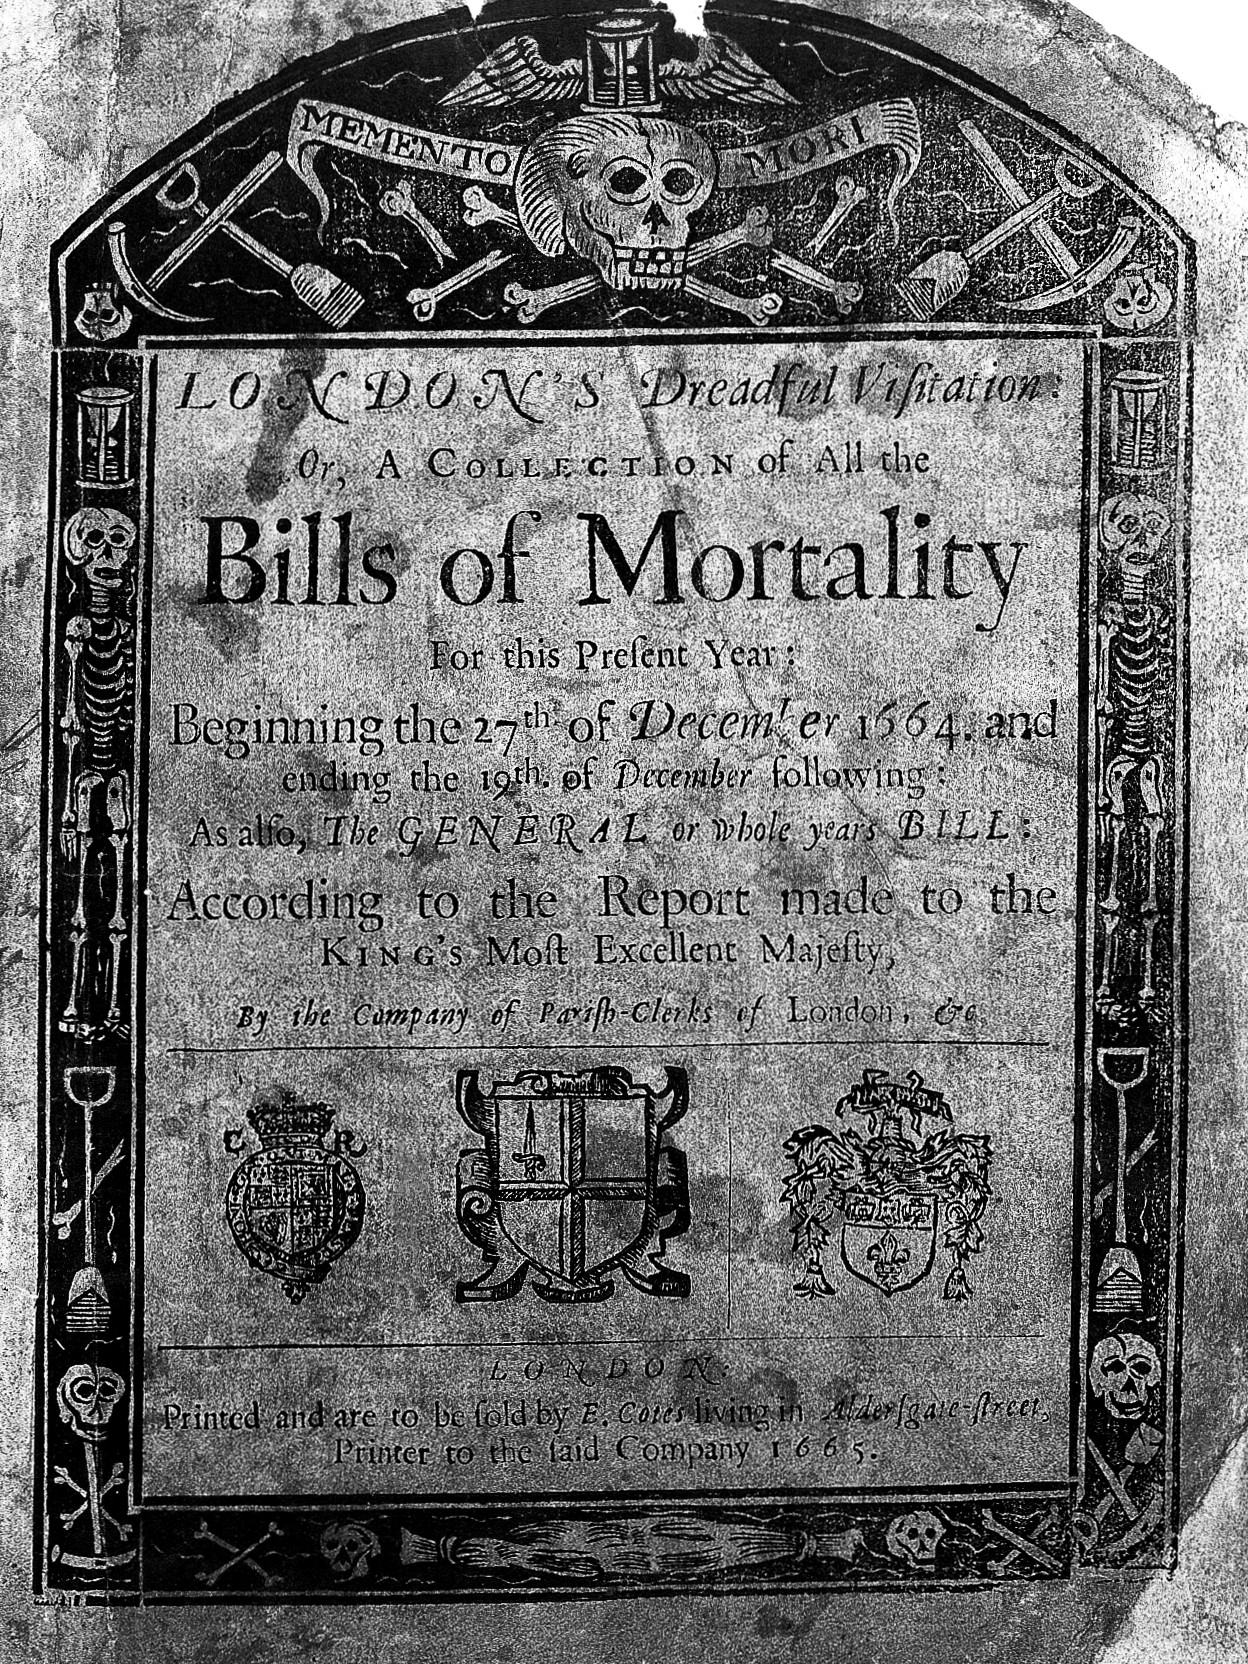
\includegraphics[width=\linewidth]{./figures/bills-of-mortality.jpg}
	\centering
	\caption{London's Bills of Mortality, 1665 (\href{https://commons.wikimedia.org/w/index.php?curid=36040989}{Wellcome Images}).}
	\label{fig:billsofmortality}
\end{marginfigure}

The reductionist scientific method was formalised and scientific institutions were established to embed this radical problem solving approach. Problem-solving was beginning to be predicated upon the 'taking apart' the object of study into its most fundamental parts. Knowledge was gained of each of the parts, which were 'reassembled' to gain knowledge of the 'whole'.

Similarly, scientifically based analyses looked at a problem, for example causes of death in London, and began to identify: how many deaths from each distinguishable cause; the age of the people who died; where they lived; their occupation, etc. Creating knowledge about deaths in the London population began by looking at each part of the problem and then compiling information to get a picture of what was happening.

\subsubsection*{Infectious disease surveillance}

Epidemiology, the science of public health, began to take form mid-nineteenth century, and with it infectious disease surveillance emerged to create the form and function of a first semblance of public health intelligence. Together they began to deliver knowledge of the natural history of disease, its etiology, and occurance, along with information on its incidence and prevalence in the community. Public health practice, as we know it today, began. Happy days!

Notifiable diseases and international standards of reporting have been happening for almost a hundred years. However, the real methodological home of public health intelligence can be found in early efforts to intervene in outbreaks of disease. One example of an early analytical approach to epidemiology and public health can be traced back to at least 1854 and John Snow's map of cholera in London (Figure~\ref{fig:johnsnow}). Thus began the tradition of investigating and reporting on infectious diseases outbreaks, which has contributed to the body of knowledge and practice that is undertaken by all developed nations and under the general rubric of 'public health intelligence' today. More importantly perhaps, the conceptual emergence of 'information for action'.

\begin{marginfigure}%
	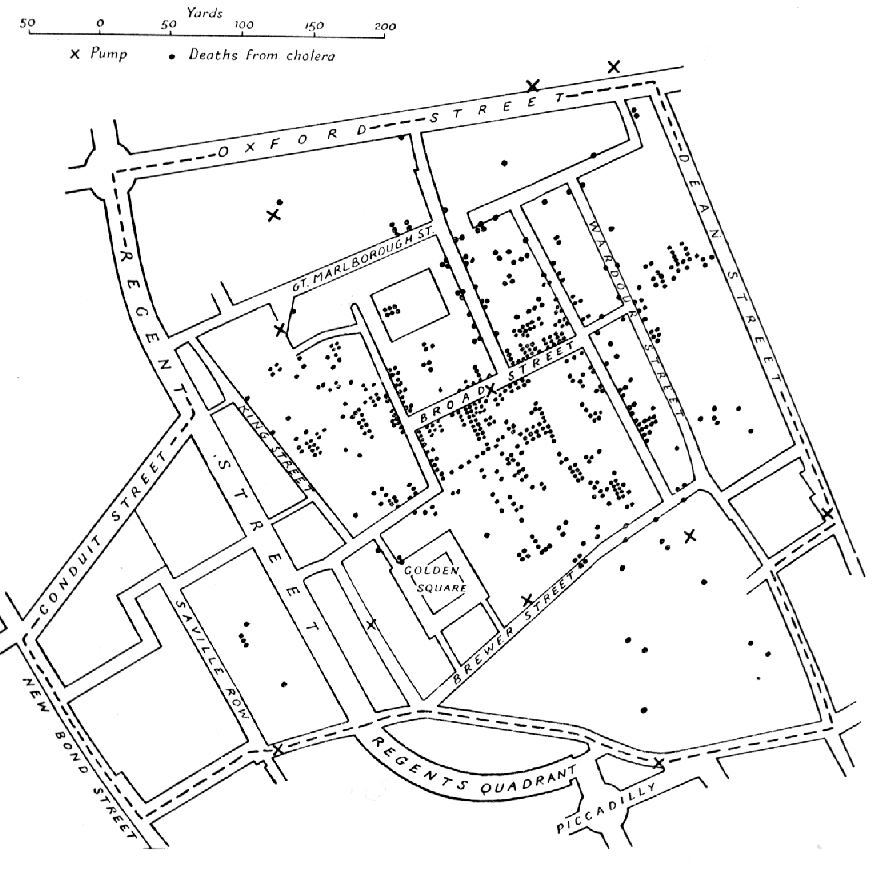
\includegraphics[width=\linewidth]{./figures/Snow-cholera-map.jpg}
	\centering
	%\bigskip
	\caption{John Snow's 1854 cholera map of London denotes the location of deaths and is a very early example of analytical thinking in health intelligence (\href{https://commons.wikimedia.org/w/index.php?curid=403247}{Wikimedia Commons}).}
	\label{fig:johnsnow}
\end{marginfigure}

\subsection{Chronic Disease and the beginning of the Information Age}
The beginning of the information age coincided with the epidemiological transition from infectious to chronic disease in most developed nations.

Public Health Intelligence (mid-20C) -- transition to chronic disease and digital data

The major developments over the last few decades have included moving disease analysis, storage and reporting from paper-based to digital systems. In my experience, a considerable portion of the public health intelligence resource has traditionally been expended on data collection and cleaning processes, not on analysis, let along insight development. Until the recent adoption of a data analytics posture, the tools of the trade had, for a long time, primarily been spreadsheets and relational databases.

\subsection*{Business intelligence and analytics}
Business Intelligence was the private sector's answer to public health intelligence, and with it began the move towards 'analystics' and away from bespoke 'analysis'.

Business Intelligence and Analytics (mid-20C) -- analytics and data warehouses


\subsection*{Data Science} 
Data Science marks the height of the analysis paradigm and so to the beginning of its decline, perhaps. We seem to have come full circle 

Data Science (early-21C) -- beginning of the end for the 'analysis paradigm'



The move to data analytics and adoption of data science methods....

Why?

\section*{Public health intelligence is falling short}
% Why is it falling short? This section title is NOT informative and all 
% sections in ToC need to be informative. I agree it is falling short, but
% why. What case is made below? Need to have a case to be made.
% Off the top of my head:
% 1. We can't see what difference we are making
% 2. PHI currently supports silo'd thinking
% 3. Although we can assess what is happening (events) and anticipate 
%    what is coming next (pattersns), we are unable to adequately analyse
%    the structure of a problem let alone the thinking that underlays that
%    ...

What is the purpose of public health intelligence? I think that most of my colleagues would phrase the response to this question something along the lines of: "The purpose of public health \emph{intelligence} is to deliver high quality \emph{information} in a timely manner to our clients to enable the development of \emph{insights} that facilitate \emph{evidence-based decision-making} that is ultimately successful." There is a bit to unpack here:

\begin{description}
	\item[Intelligence:] A product or activity/function that delivers contextualised information in response to a challenge or question
	\item[Information:] Data with sufficient structure to enable its use in getting 'business' (aka public health interventions) done
	\item[Insights:] An interpretation of information leading to an increase in understanding
	\item[Evidence-based decision-making:] Public health practice is predicated upon the belief that this is what we do, even when sometimes this is questionable
\end{description}

Earlier in the history of public health, prior to the development of an explicit 'intelligence function', disease surveillance teams termed what they did as providing 'information for action'. Despite the broader range of foci across current intelligence functions, this ambitious purpose could be reinterpreted as "intelligence for action". However, public health intelligence appears to be focussed on a much less ambitious goal than earlier infectious disease surveillance efforts had in mind, i.e. 'information for action'(Figure~\ref{fig:IntelLM}).

\begin{figure}
	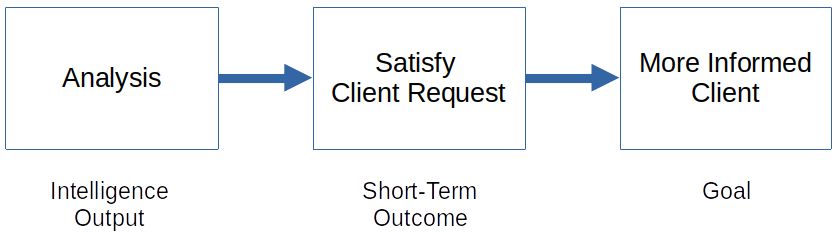
\includegraphics{./figures/Current Intel Logic Model.png}
	\caption[Current PHI Theory-of-Change][6pt]{A simple theory-of-change captures the essence of much of current public health intelligence practice: Do the analysis to satisfy client requests with a view to having a more informed client at the end of the process.}
	\label{fig:IntelLM}
\end{figure}

Indeed, I believe that public health intelligence needs to readopt 'action' as a goal (Figure~\ref{fig:toc}). There may be a couple reasons why we currently don't have the same focus on 'action' that we used to, but they come down to the complexity of communities in which public health is trying to take action. It's not just about 'removing the pump handle'. Chronic disease interventions may require years to demonstrate a result. The result, if there is one, may be masked by other noise within the system and be hard to attribute to the intervention(s).

However, I think that there is also another factor at play, one that we don't discuss very often -- the very nature of public health organisations. Compared with early efforts that were almost entirely focussed on infectious disease interventions, we now have a large number of areas that we try to influence. Therefore, we attempt to 'divide and conquer problems. We create silos, even silos within silo of efforts and domain knowledge. Public health intelligence is a silo. Those who do analysis do not, as a rule, also build and deliver public health interventions. Perhaps the most defining characteristic of public health intelligence is that analysts answer 'client' questions -- that is the new goal.

Public health intelligence analysts are specialists. Epidemiologists also specialise in particular diseases or transmission modes or populations at risk, in ways similar to the specialisation of the medical profession. Analyst participation in public health engagement, planning and action cycle is generally limited to three stages of client request clarification, data processing and analysis  (Figure~\ref{fig:AnalystCycle}).

\begin{figure}[t]
	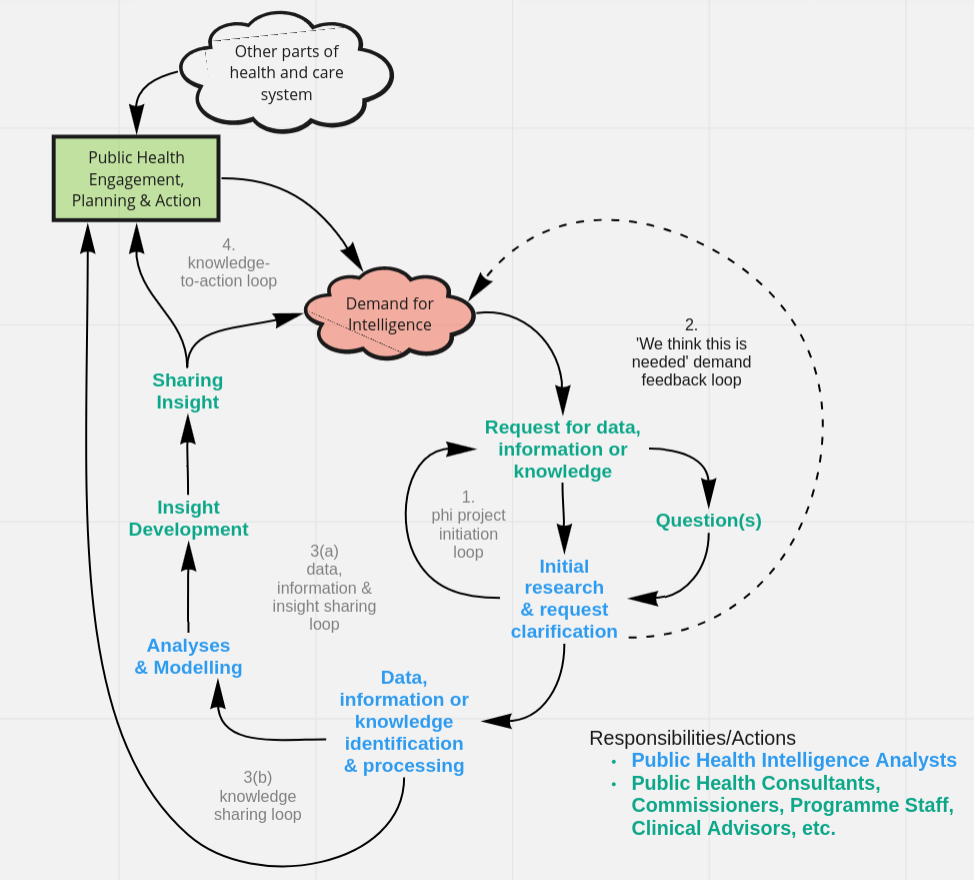
\includegraphics{./figures/PHI Analyst Cycle Draft.png}
	\caption[Current PHI Analyst Cycle][6pt]{DRAFT. Demand for public health intelligence creates a number of feedback loops defining relationships with their public health 'clients'.}
	\label{fig:AnalystCycle}
\end{figure}

Specialisation can be very useful for increasing the efficiency of processes, particularly where advanced analytical skill sets are limited and therefore need to be used to best effect. The problem underlying the request for intelligence is most often quite opaque to the analysts. This is true for a number of reasons that include time pressures, lack of analyst health domain knowledge, the inaccessibility of decision-making forums. It doesn't really matter why we can't see and/or understand 'a client' problem, but the end results is we usually have a fairly incomplete picture of the intelligence need, and means that we can easily be working on the wrong problem.

\begin{marginfigure}%
	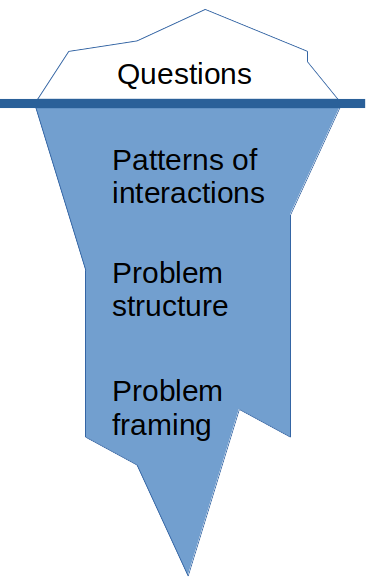
\includegraphics[width=\linewidth]{./figures/PHI Iceberg.png}
	\centering
	%\bigskip
	\caption{Edward Hall's Iceberg model is used here in an attempt to better understand the things we can't easily see about the public health intelligence process.}
	\label{fig:iceberg}
\end{marginfigure}

\subsection{Client questions and problems}
Clients ask analysts questions and analysts try and answer those questions, but if all an analyst can see is the question, they do not have a big enough picture to ensure that they are answering the right questions. Questions are therefore what the analyst sees, like an iceberg (Figure~\ref{fig:iceberg}). It is what remains out of sight, ie. below water that remains dangerous, and while an analyst can infer much about the problem through repeated engagement with clients over time, the analyst rarely develops sufficient knowledge about the structure and framing of the problem. Therefore, the extent of the danger of the hidden iceberg and of not answering the right question remains.

Ultimately, only decision-making that is underpinned by science is deemed acceptable in most modern health and care systems. Science, aka scientific reductionism, is the theoretical basis for the analysis process. Consequently, the analysis paradigm has been the only approach available to most analysts.

Indeed, most of us are Analytical Thinkers. This paradigm is so engrained that when we consider the meaning of the term 'thinking', we are actually describing 'analytical thinking'. That shouldn't be surprising as this paradigm has been at least 400 years in the making, deriving from  the reductionist scientific approach to problem solving and knowledge acquisition. The science under-pinning most of public health is epidemiology, and epidemiology is a reductionist scientific discipline.

\subsection{Ackoff's description of analytical thinking}
'Analytical thinking' is a term created by the organisational theorist, Russel Ackoff, to describe the paradigm by which we attempt to solve problems. We respond to problems or challenges identified by our organisation using Analytical Thinking in three basic steps (Table~\ref{tab:analysisthinking}).

\begin{table}[h]
	\begin{center}
		\footnotesize%
		\begin{tabular}{p{4cm} p{6cm}}
			\toprule
			Process & Example  \\
			\midrule
			Step 1: Disaggregate problem & CVD deaths into deaths by sex, age, co-morbidities, deprivation\\
			Step 2: Examine each part & Statistically describe and analyse of patterns\\
			Step 3: Reassemble for an understanding of the whole & Model the relationships between risks and outcomes\\
			\bottomrule
		\end{tabular}
	\end{center}
	\caption{Russell Ackoff's three step process defining 'Analysis Thinking'.}
	\label{tab:analysisthinking}
\end{table}

This process is the dominant paradigm in health intelligence, and it has served us well for many decades\cite[-1\baselineskip]{RegmiandGee2016}. However, we also know that working with clients to identify the ‘intelligence challenge’ and any underlying questions is often a long iterative process. It is often unsatisfying because the ‘client’ often does not want to invest a lot of their time – ‘they just want the data’ (actually they want information, but let's not quibble).

However, our ‘single minded approach’ to health intelligence is largely responsible for the difficulties we experience in effectively engaging with clients – there appears to be only one way to support decision-making and that’s through Analytical Thinking (Figure~\ref{fig:at1}).

\begin{figure}
	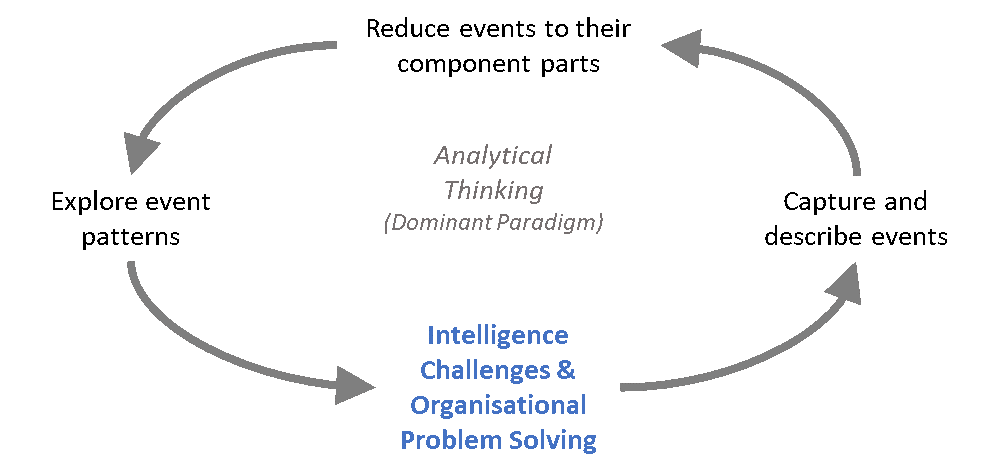
\includegraphics{./figures/analytical thinking feedback loop.png}
	\caption[Analytical Thinking is powerful][6pt]{Analytical thinking, while increasingly powerful through the adoption of data science methods, nonetheless provides a single approach to organisational problem-solving and the support of decision-making.}
	\label{fig:at1}
\end{figure}

The domination of Analytical Thinking over any other type of approach to problem-solving didn’t happen by accident, it is a product of the very successful reductionist scientific approach (Figure~\ref{fig:at2}). The problem we now have, and most analysts sense this, is that what worked well for understanding diseases, viruses and the like, doesn’t quite deliver the same understanding when applied to health systems where human decision-making, organisational culture and complex inter-organisational structures create complexity and dynamics/behaviours. This is our ‘problem-solving’ space.


\begin{figure}
	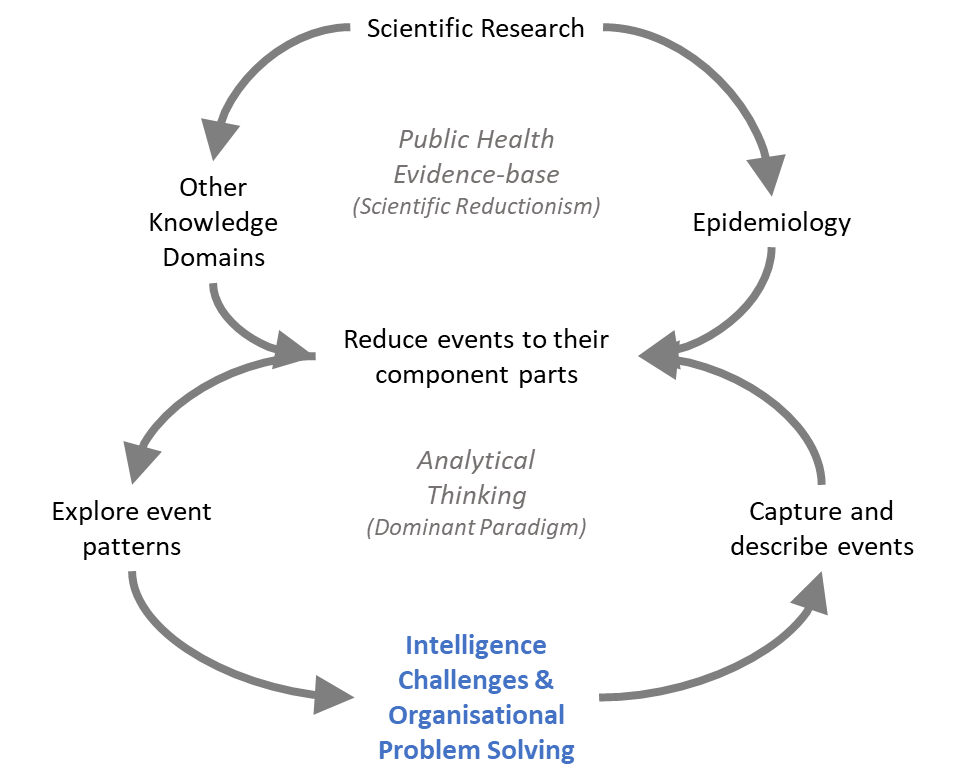
\includegraphics{./figures/analytical thinking reductionist science.png}
	\caption[Analytical Thinking is reductionist science[6pt]{Analytical thinking is driven by the same reductionist processes that are at the heart of most scientific research. This approach to problem-solving has been hugely successful delivering the ‘public health evidence-base’, but it is limited in what it can explain about the functioning of systems that include human behaviour, e.g. health systems.}
	\label{fig:at2}
\end{figure}

\subsection{Two Key Public Health Intelligence Challenges}

To be sure -- public health intelligence has many challenges, but I think two challenges are fundamental as they speak to the effectiveness of this critical function.

\begin{enumerate}
	\item Operational Challenge: Every public health intelligence group struggles with 'client engagement' that is centred around identifying and articulating what it is that the client really needs.
	\item Strategic Challenge: The bigger picture problem is that in most organisations, the intelligence function is limited to gathering, managing and analysing data. I think that this is a very short sighted view of the 'intelligence function' and what we really ought to be doing to be focussing on is working with colleagues to solve organisational problems, not fling data all about , which is mostly counter productive.
\end{enumerate}


\section*{Why preventing ill health seems beyond our ken}

Analytical thinking has had its day, it transitioned us away from the 'dark age' into a period of 'enlightenment'. Problem solving from the Renaissance onward has be dominated by reductionist scientific thought that has delivered massive advances in knowledge and technology. It created the 'machine age' and later the 'information age'. Knowledge continues to rapidly grow today, and yet there are more and more global and local problems that we can't solve: Climate heating, environmental degradation, loss of biodiversity, war, poverty, inequality, population health, healthcare affordability. The list is seemingly endless.

It could be argued of course that we choose not to solve many of these problems, not that we can't solve these problems. There is certainly a whiff of that in our political, social and cultural lives. Nonetheless, I think that most people would identify these as problems to be solved. Many writers have suggested that we are currently transitioning from the 'information age' into the 'systems age', and that our approach to thinking and problem solving needs to follow, if we are to continue solving real-world problems.

\begin{itemize}
	\item when did things get too complicated?
	\item R Ackoff quote about a scientific conference in late 1800s where they thought they would have a complete explanation of everything
\end{itemize}

Operationally, public health intelligence needs to reassess it's engagement will clients. I think we need to change from an 'intelligence as service' posture to an 'intelligence as a consultancy' posture where we (a) acknowledge that our public health colleagues are just as important to the intelligence function as are the analysts, in fact they are an integral component of the intelligence function (we just pretend that they aren't); and (b) we need to think differently in a number of ways, but most importantly we need re-engage the public health workforce with 'systems thinking' and we need to co-design the intelligence delivery.

Strategically, public health intelligence should refocus on supporting organisational problem solving. Population health intelligence does not in and of itself improve the health of the population. Surely, this is self-evident to most people? However, just to reinforce the above quote and differentiate population health intelligence from activities that have the potential to change the health of the population: 

\begin{adjustwidth}{3em}{0em}
	\begin{description}
		\item[public health interventions] can improve population health;
		\item[sound public policy] can improve population health;
		\item[reducing poverty] can improve population health;
		\item[decreasing inequality] can improve population health.
	\end{description}
\end{adjustwidth}

If public health analysts do not do these things, how then can we use population health intelligence to improve the health of our populations? For a start, we need to stop working in silos. An oft repeated mantra in some quarters, but how do we actually achieve it? The second change we need to make and this maybe seen as heresy in some quarters, but we need to stop focusing on 'intelligence' and start focusing on 'problem-solving'.

Inscribed on Marx's tomb is the following very apt challenge to public health analysts (except he was speaking of \emph{philosophers}), and perhaps, we should incorporate this challenge into our building systems-based public health practice, as

\quotation{%
	\centering
	The \emph{analysts} have only interpreted the world, in various ways.\linebreak The point, however, is to change it.\footnote{\href{https://en.wikipedia.org/wiki/Tomb_of_Karl_Marx}{Wikipedia:} Karl Marx's Tomb}
}

% Left over from a former section 3.2 in next Chapter -- wasn't a good fit 
% after the last rewrite

Let me start with a different question, since most of us are first and foremost (if not solely) analysis thinkers -- what makes 'good analysis practice'? Here are some thoughts
\begin{itemize}
	\item You know how to formulate problems in a manner that allows to you analyze them
	\item You are able, from knowledge of the problem (business need) and of analysis methodology, to match problems to method
	\item You are also able to adjust methodology based on the nature of the data you have available and appreciate the limitations of methods and data
	
	\item You are able to process data into suitable formats for analysis
	\item If you are suitably experienced you are able to interpret the results of analyses that you or other perform
	\item You are able to apply these insights and/or communicate them to others such that the analysis is useful to the organisation
\end{itemize}



\section{If you aren't here for a simple answer, buckle up for the ride out of 'old thinking'!}

The practice of public health is core business for only a few of us. However, we have many colleagues outside of public health who are actively engaged with public health practice (health sector colleagues, academics, social care, etc.) or who at least have an identifiable role to play in the delivery of public health outcomes (including environmental practitioners, hospitality workers, those in administrative and management roles, etc.)\footnote{While the 'few of us', in the UK, is probably more than 40,000, we also have more than 14 million colleagues with a direct role to play. That's a lot of us and we work in many organisations, health systems, and sectors! Source: Centre for Workforce Intelligence. July 2015. Understanding the wider public health workforce, GOV.UK}.

Public health analysts and decision-makers at all levels, I'm writing this for you. If, like me, you feel that something is missing or that you aren't getting the impact from your organisation's intelligence function that you need, then maybe what follows will be food for thought, maybe even useful.

I am speaking directly to my public health colleagues about the public health intelligence function. More broadly, I would expect that this content may also resonate with public service colleagues outside of health because I suspect that they face similar intelligence challenges. If you are a problem-solver, I hope that this book is welcome food for thought and I certainly welcome your thoughts in return\footnote{The best way to reach out to me is through my (\href{https://www.linkedin.com/in/wchrrisskelly}{Linkedin Profile}). I'm interested in any constructive thoughts, feedback or genuine conversations on the topics within\ldots}.

For those colleagues who see public or population health intelligence in a more traditional light, focussing on collecting, processing and analysing of numerical data, then you'll be disappointed with the very shallow to non-existent treatment of those topics in this book. The 'bills of mortality' have been done to death (pun intended). Nonetheless these are still important topics inasmuch as we still seem to get these analyses wrong, and their data science equivalent data analytics wronger (not a word, but this too was intended). However, if you want to understand why we get them wrong and how we can fix them, then please follow along, as we will be exploring this aspect of the 'traditional' population health intelligence process.



\section*{How to move your organisation towards a systems-based practice}

\begin{enumerate}
	\item Understand where we are now -- Analysis Paradigm
	\item Develop a cognitive model for systems based practice
	\item Implement systems based public health practice
	\item Create organisational learning to power the transformation
\end{enumerate}

This story has a main four parts. However, the first three parts are set out 'from outside in', and like an onion we have a look at each and peel them away in order to appreciate the next layer (Figure~\ref{fig:apptosensemaking}). You may also notice that, at least for analysts, that this is from least familiar to most familiar. However, and perhaps most importantly, we are dealing with biggest picture first in futures thinking---the business needs, which is all too often forgotten in the rush to crank the handle and produce data, analytical thinking, which we'll deal with last.

The first part, futures thinking, is big---hopefully infinite. It relates to our business need, which in population health intelligence is very big indeed. If you work in a hospital your business needs are defined by your patients, staff, healthcare services, legislation, regulation, contractual obligations, infrastructure, health outcomes, etc. The key bits for an analyst to consider:
\begin{itemize}
	\item You should know that the business need associated with every request for intelligence, but if your intelligence process is treated like Mr Ford's first assembly line, you might not. If that's the case, you are missing a big chunk of being able to create intelligence for action. It is 'why' you are trying to answer the question (if are lucky enough to have one of those) in front of you.
	\item Analysts have plenty of skills that can be used to understand and articulate business needs.
	\item Business needs don't stay the same, ever. The world changes.
\end{itemize}

The second part we look at is systems thinking. Systems thinking is big too. Maybe not as big as futures thinking, but systems thinking is focussed on the here-and-now. Systems thinking can certainly be used to understand business needs, but it can also be used to identify and frame the exact questions we should be asking from the intelligence process. I can't be the only analyst to have ever worked with colleagues who didn't seem to have a question and after much iterative effort discovered that:
\begin{itemize}
	\item the question has already been answered
	\item the wrong question is being asked
	\item that there really is no question
\end{itemize}

The third part of this onion is analytical thinking. This comes last, because you already know about this one, or at least you should know about this type of thinking---its what you do every day. It is our dominant problem-solving paradigm, and it used to work really well until, well it stopped providing solutions that stick. We'll have another look at this type of thinking, we'll discuss why it doesn't work particularly well on its own anymore---particularly for decision-makers, who might also not realise that it isn't working particularly well anymore.

The fourth and last part is about how we integrate these three approaches to the provision of intelligence in order to build problem-solving capability within our organisation or health system. It's less about intelligence process and method, and more about organisational development to achieve better population health intelligence.

\marginnote{
	\newthought{Key Message:} Public health attempts to create change within communities to protect and improve the health of those populations. In this, it is guided by public health intelligence activities that are entirely focussed on turning data into useful information that can guide these interventions. These are evidenced largely from epidemiology, a reductionist science. Consequently, if your problem cannot be understood and solved by breaking it into smaller parts, understanding each part on its own, then you have a major limitation.}

I've spent many years working in public health intelligence. Its been a passionate intellectual pursuit since at least the mid-1990, a period during which I was peripherally involved in the response to dengue outbreaks in North Queensland, Australia. So when I say that the 'analysis paradigm' -- the fundamental way we think, act and learn about things like disease outbreaks -- constrains past public health practice. I expect to be looked upon as a heretic. I'm as invested in this paradigm as are any of my public health colleagues.

I chose the word 'constrain' quite carefully though. Heretical is one thing, being burnt at the stake is quite another! Seriously though, I don't think for one moment that our current practice of public health hasn't benefited our communities. Of course it has and it will continue to benefit society at large; it's just that it's effectiveness is declining as complexity increases. We are still using a 19th century approach to problem solving.

I'm devastated for the same reason many of my intelligence colleagues are -- we can't see that we are having an impact any more. However, I'm also amazed, because unlike many of my colleagues I can now clearly see why this is the case.

The challenge in being able to see the problem is not a simple one, it involves: (1) evaluating whether we are indeed having an impact and to do this (2) what would this 'positive impact' look like? I have only ever tried to evaluate this once, a study of the key workforce issues for public health intelligence analysts across a region of England (Appendix~\ref{ch:case_study_3}). 

We found that our inability to see whether we are 'making a difference' could be a prime driver of job dissatisfaction. If I hadn't also been looking deeply into systems thinking, I might have left it at that. Can't see impact. Unhappy. Do something else outside public health. I know that I'm not the only person in public health intelligence who feels like this sometimes. It is a growing feeling amongst many colleagues and we should be worried about it.

However, what we see are three feed back loops (Figure~\ref{fig:SWAnalysts}). Two of these feedbacks, organisational learning and intelligence delivery appear to be reinforcing loops, which means that when things are getting better they tend to keep improving and when things are getting worse, they keep getting heading in that direction. Job satisfaction is definitely declining amongst the analysts we interviewed.

\begin{figure*}
	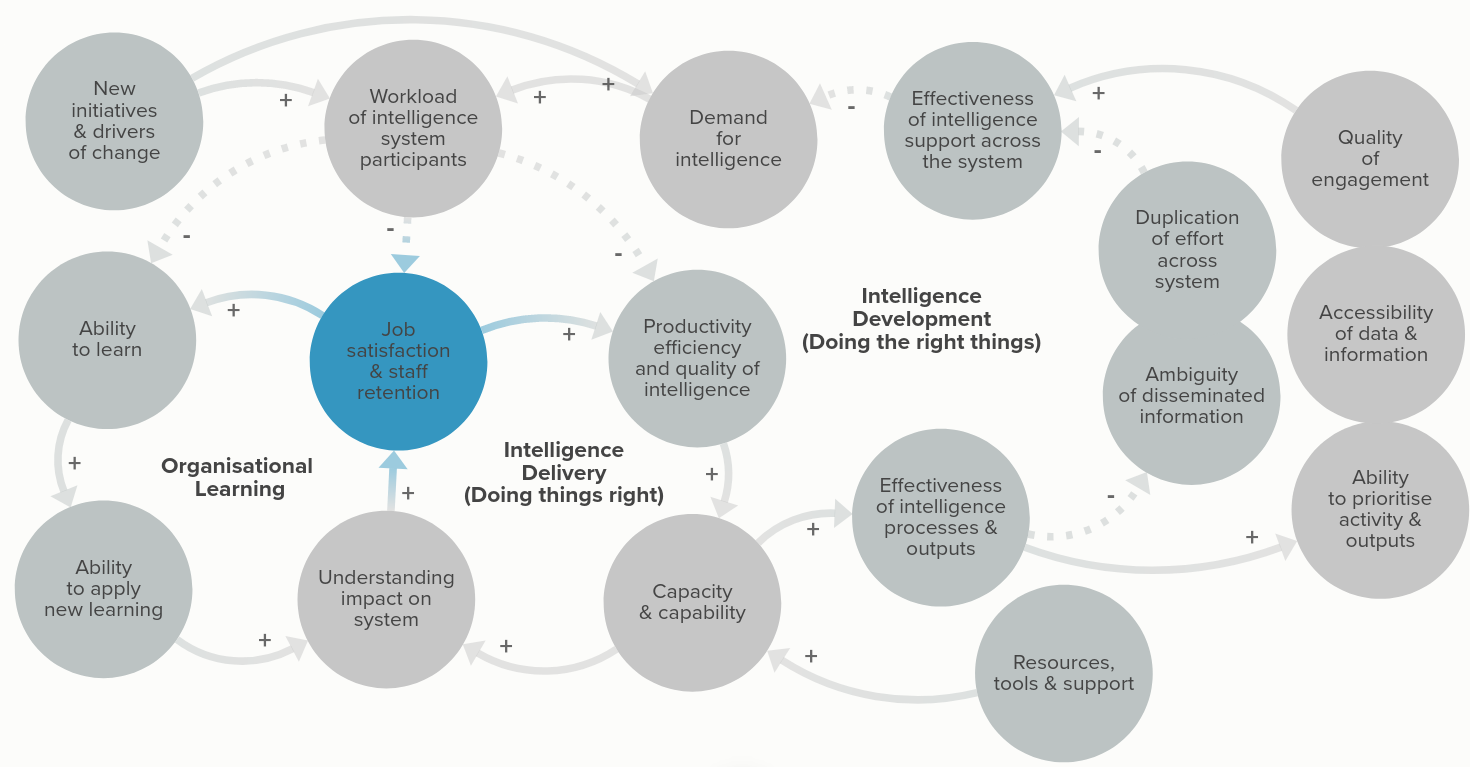
\includegraphics{./figures/SWAnalystChallenge.png}
	\caption[Public health intelligence effectiveness][6pt]{A causal loop diagram illustrates three feedback loops in regional intelligence that are likely reducing the effectiveness of public health intelligence.}
	\label{fig:SWAnalysts}
\end{figure*}

A third feedback loop, intelligence development, is much more messy, but it is of most interest to me. Its about effectiveness of public health intelligence. Does it make a difference -- so it speaks to the central question here! The feedback loop suggests that unless we have an increasingly effective system of public health intelligence demand for intelligence will continue to grow (because it isn't be satisfied), workloads will continue to grow (beyond what is manageable), and analyst job satisfaction will continue to grow with all the flow-on effects illustrated.

What I can now see is that the complexity of society in general would never all us a clear view of our impact, and this is true for public health as a whole. Population health and its improvement is never going to be easy to see or attribute blame or credit to a single effort. One only has to consider the case for smoking and cancer and heart disease. Slam dunk, right? Consider how many years public health has been on the case, how many interventions have been required (taxation, regulation, legislation, education, treatment, etc.). We've thrown everything at this and we were rewarded with initial years of decrease followed by a levelling of the trends and now projected increases. What is going on?

Complexity. Complexity is what's going on. Our view of population health has been constrained by complexity. Our practice of public health has similarly been constrained by complexity. Consequently, public health practice is primarily reactive in nature with at best some short-term ability to anticipate what is coming next. Emphasis on 'short-term'. At the heart of our inability to 'see' is the current practice of public health intelligence, which despite huge advances in analytical methods, is only incrementally improving practice.

This chapter sets out past and current public health practices as underpinned by public health intelligence activity. The current contraints in practice cannot be solved by incremental improvement, and require a new approach. What follows is the story of how we got into this situation and what it means.


\subsection{The journey out of the analysis thinking}

Absolutely everything I looked at over the next 20 years seemed to be complex, and almost nothing in my university education equipped me to apply science and analytical skills to support the resolution of problematic situations in the real world... (new para or subsection) earth observation science... (new para or subsection) climate impacts science... (new para or subsection) academia heaven and hell... (new para or subsection) Dengue!
